% Chapter 1

\chapter{Background} % Main chapter title

\label{Chapter2} % For referencing the chapter elsewhere, use \ref{Chapter1} 
\newpage

\section{Advertising}

Everywhere is advertisement of something, some event or a product and it is meant to provide the audience information about those things and gain the planned goals and effects from the specific target audience, it is a mean of mass communication that is created to alter the audience’s behavior and attitude \cite{advertisementdef}. In particular Kotler and Keller defined the advertisement as bellow

\begin{snugshade}
\textbf{Defination: Advertising }\\ \\ ``\emph{Advertising is any paid form of non-personal presentation and promotion of ideas, goods, or services by an identified sponsor. Advertisers include not only business firms but also charitable, nonprofit, and government agencies}''\cite{ad_def}.
\end{snugshade}

So based on the definition above advertisement is non-personal meaning it is meant to a group of people or target groups, secondly it should represent an idea or basically it should have something to deliver for the people which matters to the audience and normally it does have sponsor(s) to launch it somewhere for example on TV, Radio or print a poster version outdoor. The way message is being delivered has been changing at every era of development as discussed bellow.



\subsection{History of advertisement}

From very old ages as from 13th century advertising has played an important role to promote customers attention and be able to compete with one another, The first paper advertisement was published at 1704 in an American newspaper called Boston News Letter, which was about houses and lands to be sold\footnote{Paper advertisements: http://infoacrs.com/a/adhistory.html, Last accessed 16th March 2016} and after that lots of business started to do their advertisements in newspapers, posters and banners. The first television ad was shown at 1941 on an American TV\footnote {First TV ad: http://www.openculture.com/2013/08/watch-the-first-commercial-ever-shown-on-american-tv-1941.html, Last accessed 16th March 2016}, this ad brought attention to a wide area of application and big business industries toward advertisement as a result the budgets raised much higher for advertisements and later advertisement entered the World Wide Web or so to say online advertising, which has evolved now to multi-billion dollar industry. Now because of the emerging new technologies and advancements, advertisements are in our smart phone applications, smart TV sets, tablet PCs and many other smart devices. And from past decades display screens are replacing print advertisements because of the easy reusability of the screen and convenient usage of them and providing dynamic contents.


\subsection{Pervasive Advertising}

Currently computers play important role in life, and it is becoming nearly common and found everywhere and these computers do not have to be like traditional computers like desktops having keyboard and mouse, it has various forms like it could be our laptop to a smart watch or even a smart pen and these technologies blend in our environments too like different kinds of displays, sensor, security cameras, fridge, washing machine and more, so as a result we have ubiquitous computing environment that is supported by underlying technologies like Internet, middleware and microprocessors, as explained by Mark Weiser \footnote{Ubiquitous Computing: http://www.ubiq.com/hypertext/weiser/UbiHome.html}  \cite{ubiquitous_computing} ``\emph{Ubiquitous computing is the method of enhancing computer use by making many computers available throughout the physical environment, but making them effectively invisible to the user}''. The term pervasive computing is also used instead of ubiquitous  \cite{pervasiv_ubiquitous} and it is constructed from basic elements \cite{pervais_ad} (1) ubiquitous access, (2) context awareness, (3) intelligence and (4) natural interaction and when advertisement is made with the help of pervasive computing which is called ``\emph{pervasive advertising}'' would really help to improve advertisement in general because of the powerful properties of the pervasive computing like ubiquitous feature that computing is integrated seamlessly in environment and it disappears, like as Mark Weiser’s \cite{twenty_first} another central statement was ``\emph{The most profound technologies are those that disappear. They weave themselves into the fabric of everyday life until they are indistinguishable from it}''. Based on above explanation, the pervasive aevertising is defined as bellow.

\begin{snugshade}
\textbf{Defination: Pervasive Advertising }\\ \\ ``\emph{Pervasive advertising is the use of pervasive computing technologies for advertising purposes.}''\cite{pervasiv_ad}.
\end{snugshade}




\subsection{K / L value}
\subsection{Metaphors}
\subsubsection{Mirrors}
\subsubsection{Windows}
\subsubsection{Overlay}
\subsubsection{Posters}

\section{Public displays}

Displays are increasingly getting cheaper and being used in various locations like restaurants, hotels, sport stadiums, homes and now in public space like shop windows, supermarkets, airport and streets and roads. Most of these displays shows advertisement in which dynamic or static content is being shown and at few of them are interactive like purchasing train tickets with a touch capability, checking in airport and even interactive advertisement in which passers-by can be engaged and play game. 
This section discusses on the history of public display, novel applications of display, sensing technologies that are being used in displays, attraction of display and how engagement is designed for displays by the design of novel interaction techniques and at the end how displays are evaluated and what are the methods and tools to do so.


\begin{snugshade}
This is based on following publications.
\end{snugshade}


\subsection{History of public display research}

Various researches have been done from the past three decades and are still continuing until today, as the first research was conducted in 1980 called the ``\emph{Hole-in-Space}'' \footnote{Hole-In-Space: https://www.youtube.com/watch?v=SyIJJr6Ldg8} that connected New York and Los Angeles one side-walk with a live video and sound system, people at both end could hear and see each other, in this research common behavior and interactions of people were explored and other similar researches had also been done.\\

Different sized displays were also designed to fit working area and space for various tasks, like Mark Weiser illustrated in his paper ``\emph{Computer for 21th century}'' \cite{ newgenerationcomputer}, in which he present tabs, pads, and boards devices which could be used as a personal use and also showed large scale displays equivalent to blackboard for public use, and demonstrated that how can these technologies be integrated as ubiquitous and be adjustable based on user demands and context. \\

Another research on situated displays that projects content based on location for-example  \emph{FLUMP}\footnote{flexible ubiquitous monitor project: http://research.cs.ncl.ac.uk/cabernet/www.laas.research.ec.org/ \\ cabernet/workshops/radicals/1996/papers/flump-finney.html, last accessed May 15, 2016.} \cite{flump}, this project was designed to research and illustrate the effectiveness and adaptability of ubiquitous computing systems. Many researches also conducted to design wearable displays like Meme tags and group tags \cite{meme-tags} that by wearing the displays participants could share ideas and opinions called “memes-succinct” among themselves, and through large display called “community Mirrors” these memetics exchanges were visualized live for conference audience. Another “Name tags or thinking Tag” from IBM \cite{ibmtags} that would show the name of the person when facing another person and also display relevant information on who is viewing the tag.\\

Furthermore, ambient displays were also researched for-example the \emph{Waterlamp and the pinwheels} used \emph{ambientRoom} of Ishii and ullmer \cite{ambient}, in which they showed how tangible bits could connect the cyberspace and physical environment and foreground and background of human activities. The room was kind of augmented space using light, sound and airflow and water movement. Another was \emph{office plant\#1} \cite{office_plant}, which was an exploration of a technological object adapted to the office ecology, another was \emph{Information Percolator} \cite{information_precolator}  this ambient display was designed to show expressions placed within decorative objects \footnote{Information Percolator : https://www.youtube.com/watch?v=9LGQWhCePc8, last accessed:16 May 2016},  Greenber and Michael \cite{shared_notes} investigated on how people transition from individual interaction to group work with the use of PDAs and shared displays and based on this they introduced SharedNotes system and illustrated how people can switch to different modes.\\

Encouraging social interaction was another important aspect for public displays, researchers like Chew and leclerc \cite{chew_interaction} focused conversation in a conference setting using display called \emph{Sparks} which ``\emph{an ambient social networking and communication facilitation interaface}'' this had interactive features on information related to elements presented in the space. Another interactive display designed for hospital \emph{AwareMedia} \cite{ interactive_hospital}, which facilitated  social, spatial, and temporal awareness and supported coordination at an operation ward. Gesture based interactions with ambient display was researched by Daniel Vogel \cite{vogel} that developed interaction framework for sharable, interactive public ambient displays\footnote{Interactive Public ambient display:  https://www.youtube.com/watch?v=aFl71SPeYto, last accessed: 16 May 2016} it could also support implicit and explicit and multi-user interactions, \emph{Blueboard} \cite{blueboard} , which was developed at IBM Research, was a display system for groups to exchange information in a walk-by situation, \emph{IM here} \cite{ imahere} by Elaine M.Haung that researched on LDGAs \footnote{Large display groupware applications} and proposed a design on how to share IM\footnote{Internet messaging} large displays by using mobile phone, this helped to be an awareness and communication tool.\\

At end of 2000s mobile phones became popular and common among people and was also a good mean of interaction with displays, \emph{C-Blink} \cite{cblink} that used mobile phone display, which was used as light source that sent various hue color to a camera from which the camera would detect and encode information and present on large display. Another approach was the use of Flashlight of phones as a pointing device as Shirazi and winkler \cite{flashlight} described the design of public-private display with flashlight simple interaction. Other features of phone like Bluetooth, Infrared were also used as an interaction mean with display (e.g., \cite{bluetooth2, Bluetooth}).\\

Consequently advertising also became a focus for researchers as Krüger and Müller illustrated their design of how to recognize passers-by via Bluetooth \cite{toward_situated} and how long did they stood in front of display or whether they read the content or not by video based face detection and by doing this the most relevant information would be presented in the screen, \emph{BlueScreen} \cite{bluescreen} which selected and displayed adverts in response to users detected in the audience,Stepping more further to give users choice of changing and reforming the content shown on display, \emph{Prospero project} \cite{prospero} that developed a display framework that could be configurable and controlled in public, \emph{RunWithUs} \cite{runwithuse} a social sport application that motivated people to do sport and share their progress, \emph{Digifieds} \cite{digifieds} another plateform that users could post ads in public displays.


\subsection{Auto-active displays}
Beside hundreds of researches on public displays, there are other displays, which were and are made by private advertisement industries and most of these displays are auto-active or non-interactive displays, these displays are situated in train station, airports, malls, restaurants and various locations mainly for advertisement purposes. \emph{zipper}\cite{zipper}at year 1928 made LED display at the front corner of the New York Times building, this display was showing current headlines, in Olympic 1979 the very first large display was deployed, which had video enabled \footnote{Olympic glory a short history of Olympic games timing. London in August 2012 http://www.runnersworld.com/olympics/a-short-history-of-the-olympic-games}






\subsection{Engagement with displays}
\subsubsection{Attention}
\subsubsection{Motivation}
\subsubsection{Interaction}
\newpage
There are many stages until users actually interact with the advertisement as shown above by Michells,D and Muller,J in the journal of HCI \cite{AudienceFunnel} Attention and motivation will eventually lead to interaction and these stages follow each other if the first step fail the rest would not happen. In this part of the study I want to focus more on the attraction attracting part of advertisement.

\begin{figure}[htp]
\centering
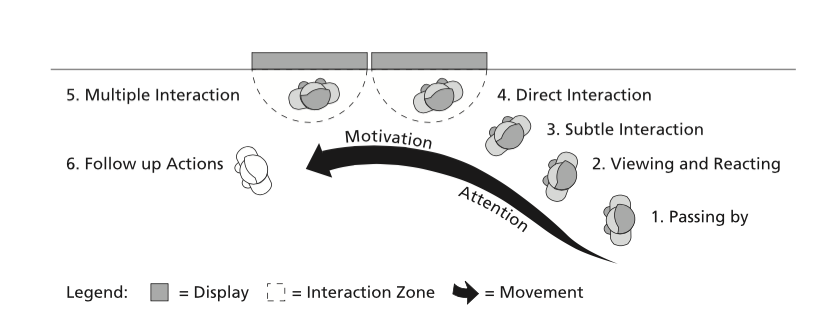
\includegraphics[width=120mm,height=70mm]{Figures/3/TheAudienceFunnel}
\caption{The Audience Funnel}
\label{fig:audience_funnel}
\end{figure}


\subsection{Interaction modalities}
\subsubsection{Body}
\subsubsection{Mobile}

\subsection{Interaction models}

\subsection{Evaluation}

\subsection{Approaches to Research}
\subsection{Methods and tools}







 





